\begin{figure}[!t]
  \centering
  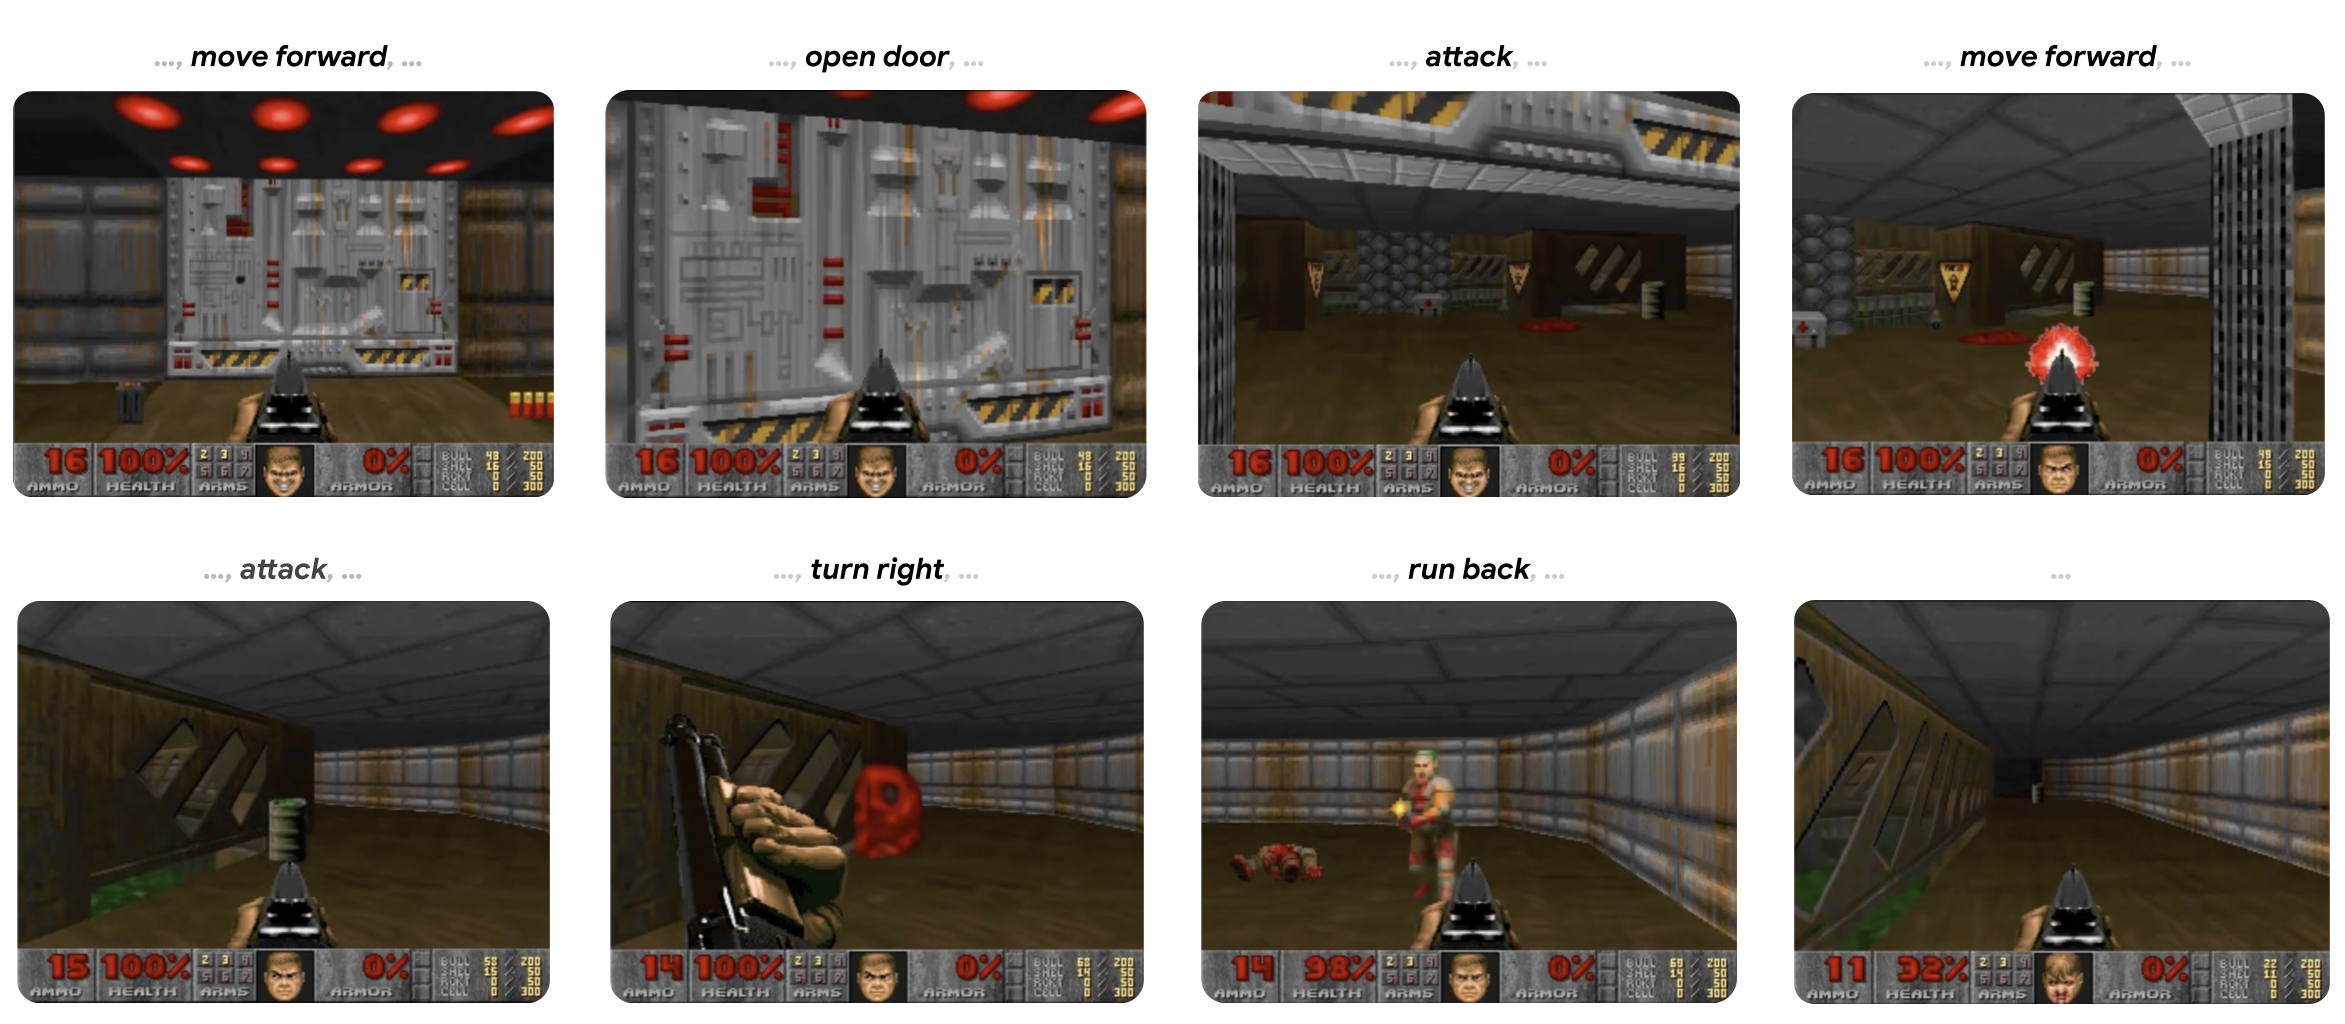
\includegraphics[width=0.98\linewidth]{fig/teaser.png}
  \caption{
The proposed methodology showcases a novel ability to produce temporally consistent and visually authentic human image animations by leveraging a reference image and a prescribed sequence of motion articulated through 3D human parametric models. 
Furthermore, it demonstrates an enhanced capacity to refine shape alignment and motion guidance within the resulting videos.
This approach facilitates the animation of a wide range of characters, encompassing portraits exhibiting substantial domain variations, such as: 
(a) a neoclassical oil painting portraying a woman adorned in a white dress and fur coat;
(b) a watercolor portrait of a woman;
(c) an oil panel painting titled ``The Queen of Armenia'', as well as characters derived from Text-to-Image diffusion models with the following prompts: 
(d) a painting of a woman in a yellow dress, heavy metal comic cover art, space theme; 
(e) a woman in a silver dress posing for a picture, trending on cg society, futurism, with bright blue eyes; 
(f) a realistic depiction of Aang, the last airbender, showcasing his mastery of all bending elements while in the powerful Avatar State.}
\vspace{-5mm}
\label{fig:teaser}
\end{figure}

\section{Introduction}
\label{sec:intro}
Recent advancements in generative diffusion models, particularly latent diffusion models, have significantly propelled the field of image animation forward~\cite{yu2023bidirectionally,zhang2023adding,zhao2022thin,li2024synthesizing}. These advancements have found broad application in virtual reality experiences, interactive storytelling, and digital content creation, resulting in the production of a plethora of sophisticated dynamic visual content.
Within the realm of human image animation, techniques typically rely on a reference image and motion guidance specific to humans, such as skeletons~\cite{wang2023disco,hu2023animate}, semantic maps~\cite{siarohin2021motion,xu2023magicanimate}, and dense motion flows~\cite{zhao2022thin,karras2023dreampose}, to generate controllable human animation videos.
In this domain, two predominant approaches prevail: those based on GANs~\cite{goodfellow2014generative,mirza2014conditional} and diffusion models~\cite{ho2020denoising,song2020score}.

GAN based methods~\cite{siarohin2019first,wang2021one,tian2021good,wang2020g3an, yoon2021poseguided, sarkar2021humangan} commonly employ warping functions to spatially transform the reference image according to input motion for generating sequential video frames. 
By leveraging the inherent generative visual capabilities of GANs, these methods aim to fill in missing regions and improve visually implausible areas within the generated content.
Despite yielding promising results in dynamic visual content generation, GAN-based approaches often encounter challenges in effectively transferring motion, particularly in scenarios involving substantial variations in human identity and scene dynamics between the reference image and the source video motion. 
This limitation manifests as unrealistic visual artifacts and temporal inconsistencies in the synthesized content.


Simultaneously, diffusion-based methodologies~\cite{guo2023animatediff,karras2023dreampose,wang2023disco,karras2023dreampose,zhang2023magicavatar} incorporate the reference image and various dynamics as conditions at both the appearance and motion levels.
By harnessing the generative capabilities of latent diffusion models in conjunction with condition guidance, these techniques facilitate the direct generation of human animation videos. 
Recent diffusion models~\cite{karras2023dreampose,wang2023disco}, grounded in data-driven strategies, notably those leveraging CLIP-encoded visual features~\cite{radford2021learning} extracted from reference images pretrained on a vast collection of image-text pairs, in conjunction with diffusion models and temporal alignment modules, have demonstrated effectiveness in addressing the generalization challenges inherent in GAN-based approaches.
Therefore, inspired by advanced methodologies such as Animate Anyone~\cite{hu2023animate} and MagicAnimate~\cite{xu2023magicanimate}, the aim of this paper is to further optimize shape alignment and pose guidance mechanisms. 


In the present study, we propose that the use of a reference image in conjunction with pose guidance, provided through sequential skeleton or dense pose data, may present certain limitations concerning both pose alignment and motion guidance.
In a progressive step forward, we advocate for the adoption of a 3D parametric human model, such as SMPL~\cite{SMPL:2015}, to encode the 3D geometry of the reference image and extract human motion from the source videos.
Firstly, diverging from approaches that segregate the representation of body shape and pose (e.g. dense pose and skeleton methods that primarily emphasize pose), the SMPL model offers a unified representation that encompasses both shape and pose variations using a low-dimensional parameter space.
Consequently, in addition to pose information, SMPL model also provides guidance on human geometry-related surface deformations, spatial relationships (e.g. occlusions), contours, and other shape-related features.
Secondly, owing to the parametric nature of the SMPL model, we can establish geometric correspondence between the reconstructed SMPL from the reference image and the SMPL-based motion sequences extracted from the source video. 
This enables us to adjust the parametric SMPL-based motion sequences, thereby enhancing the motion and geometric shape conditions within latent diffusion models.
Thanks to the generalization of SMPL to different body shapes, we can effectively handle the substantial variations in body shapes between the reference image and source video.





Incorporating the SMPL model as a guiding framework for both shape and pose within a latent diffusion model, our methodology is structured around three fundamental components:
1) The sequences derived from the SMPL model corresponding to the source video are projected onto the image space, resulting in the generation of depth images, normal maps, and semantic maps that encapsulate essential 3D information. 
The depth image plays a critical role in capturing the 3D structure of the human form, while the normal map enables the representation of orientation of the human body. 
The semantic map aids in accurately managing interactions between different components of the human body during the process of animation generation.
2) Our analysis demonstrates that incorporating skeleton-based motion guidance enhances the precision of guidance information, particularly for intricate movements such as facial expressions and finger movements. 
As a result, the skeleton is maintained as an auxiliary input to complement the aforementioned maps.
3) In the process of integrating depth, normal, semantic, and skeleton maps through feature encoding, the employment of self-attention mechanisms facilitates the feature maps, processed via self-attention, in learning the representative saliency regions within their respective layers. 
Such multi-layer semantic fusion enhances the model's capability to comprehend and generate human postures and shapes. 
Finally, the inclusion of these multi-layer feature embeddings conditioned on a latent video diffusion model leads to precise image animation both in pose and shape.


Our proposed methodology has been evaluated through thorough experiments using the popular TikTok and UBC fashion video datasets, showcasing its effectiveness in improving the quality of human image animation.
Furthermore, we have conducted a comparative analysis of our methodology against state-of-the-art approaches on a novel video dataset gathered from diverse real-world scenarios, demonstrating the robust generalization capabilities of our proposed approach.
% In particular, the integration of a straightforward motion guidance mechanism leveraging the SMPL model can seamlessly complement many of the existing latent diffusion-based methodologies.